
\documentclass[a4paper,UKenglish,cleveref, autoref]{oasics-v2019}

\bibliographystyle{plainurl}
\usepackage{booktabs}
\usepackage{fancyvrb}
\fvset{fontsize=\small,commandchars=\\\{\}}


\def\ourtitle{Semantics of Implicitly Timed Musical Events}
\title{\ourtitle}
\titlerunning{\ourtitle}

\author{Pedro M. Silva}{Dummy University Computing Laboratory, Portugal \and My second affiliation, Country \and \url{http://www.myhomepage.edu} }{johnqpublic@dummyuni.org}{https://orcid.org/0000-0002-1825-0097}{(Optional) author-specific funding acknowledgements}

\author{José João Almeida}%
       {Algoritmi, Departamento de Informática, Universidade do Minho, Braga, Portugal}%
       {jj@di.uminho.pt}%
       {https://orcid.org/0000-0002-0722-2031}
       {}

\authorrunning{Pedro M. Silva and J.\,J. Almeida}
\Copyright{Pedro Miguel Silva, José João Almeida}

\begin{CCSXML}
<ccs2012>
<concept>
<concept_id>10010147.10010178.10010179.10010186</concept_id>
<concept_desc>Computing methodologies~Language resources</concept_desc>
<concept_significance>500</concept_significance>
</concept>
</ccs2012>
\end{CCSXML}

\ccsdesc[500]{Computing methodologies~Language resources}

\keywords{Umbundu, Angola Languages, Morphological Analysis, Spell Checking}

\funding{This research was partially funded by Portuguese National funds
(PIDDAC), through the FCT – Fundação para a Ciência e Tecnologia and
FCT/MCTES under the scope of the projects UIDB/05549/2020 and
UIDB/00319/2020.  Bernardo Sacanene acknowledges from the Angolan
govenment his PhD grant, through INAGBE (Instituto Nacional de Gestão
de Bolsas de Estudos).}

%\nolinenumbers %uncomment to disable line numbering

%Editor-only macros:: begin (do not touch as author)%%%%%%%%%%%%%%%%%%%%%%%%%%%%%%%%%%
\EventEditors{John Q. Open and Joan R. Access}
\EventNoEds{2}
\EventLongTitle{42nd Conference on Very Important Topics (SLATE 2020)}
\EventShortTitle{SLATE 2020}
\EventAcronym{SLATE}
\EventYear{2020}
\EventDate{December 24--27, 2020}
\EventLocation{Little Whinging, United Kingdom}
\EventLogo{}
\SeriesVolume{42}
\ArticleNo{23}
%%%%%%%%%%%%%%%%%%%%%%%%%%%%%%%%%%%%%%%%%%%%%%%%%%%%%%

\begin{document}

\maketitle

\begin{abstract}
  In this paper, we'll discuss a simple approach to integrating musical events, such as notes or chords, into a programming language. First we'll analyze the problem and its particular requirements. Then we will discuss the solution we developed to meet those requirements. Finally we'll analyze the result and discuss possible alternative routes we could've taken.
\end{abstract}



\section{Introduction}
Programming languages are sometimes described as data plus code. Some of that data is ingested through IO (like keyboards, files, sockets and others). Some of that data is generated by algorithms at runtime. But there's also a third category that blurs the line between data and code: literal values.

Virtually every popular language nowadays has custom syntax to allow the programmer to describe some very common (and primitive) data types, such as numbers, booleans or strings. Many modern languages even have syntax for more advanced data structures, such as arrays and dictionaries (or hash tables).

When we cross into the territory of DSLs \textit{(Domain Specific Languages)}, there is an even bigger multitude of custom syntax for the most varied data types. In this paper we will discuss one possible way of of describing musical events (such as notes, chords or rests), and more importantly, musical arrangements and melodies. We will see how to treat these structures as data values that can be integrated into a programming language.

Such problem can be divided into two parts: the syntax used for describing the notes and the operators the compose them; and the semantics of the generated events, how they are stored in memory, and how their temporal properties are handled without forcing the programmer/user to manually type them. The former is a relatively easy problem, and to minimize the learning curve for new users, we adopted a simplified version of the very popular note declaration syntax from the ABC Notation project\cite{AbcNotation}, with some minor changes. The latter is the one we'll be discussing in greater detail.

The simplest way of generating such musical events is to use already common, \textit{low-level}, programming mechanisms, such as using a procedural approach where the user creates each event manually by calling a function and providing as parameters all the events' information, such as it's timestamp and duration. This is the approach used by some of the existing languages in this space, such as \textit{SonicPi}.

\begin{lstlisting}[caption={Example of a hypothetical imperative API for creating events},label=list:8-6,captionpos=t,abovecaptionskip=-\medskipamount]
play_note( 0, 100, 'A' );
play_note( 100, 50, 'B' );
play_note( 150, 200, 'C' );
\end{lstlisting}

Instead we will take a look at a more \textit{functional} approach with custom syntax and operators. Musical events are treated as sequences, anc as such can be stored in variables, passed around and trasformed. For musical events, we will be exploring a way to define them in code, as \textit{musical literals}.

\begin{lstlisting}[caption={Our proposed declarative syntax that calculates timings implicitly},label=list:8-6,captionpos=t,abovecaptionskip=-\medskipamount]
play( A B/2 C2 );
\end{lstlisting}

But more that just being able to define those events, we will also be interested in exploring how well they integrate with existing and common programming language constructs, like variables, functions, loops and other control structures.

\section{The Problem and its Requirements}
There are two important requirements we need to consider when evaluating possible solutions to this problem: the ability to produce music interactively, and to produce music lazily.

The first requirement, \textbf{interactivity}, relates to our goal of not only being able to generate music offline, but also in a live environment: give the user the ability to program several snippets of musical events, and then control them through a virtual keyboard or through other interactive means.

The second requirement, \textbf{laziness}, refers to a concept that is familiar in functional programming languages: values are generated when we need them, not earlier. In our case, this implies that a musical sequence could be potentially infinite (like an infinite repetition of some arrangement). If playing this music live, the musician could determine to stop this arrangement sooner or later.

Given these two requirements, we can conclude we \textbf{cannot} generate all music events at the start and then sort them to play them in order. We conclude that the events must always be sorted already.

\begin{lemma}[Total Order]
\label{lemma:total-order} All operators must return a sequence of events in respecting our time unit's total order.
\end{lemma}

\paragraph*{Data Model}
The basic premise is that expressions can generate a special data type: \textbf{Music}. Music is simply a sequence of ordered musical events.

A musical \textbf{Event} can be one of many things, such as a \textit{note}, a \textit{chord}, or even more implementation-specific events like MIDI messages. While all events must have a start time, some events can be instantaneous (events with a duration of zero).

%\begin{itemize}
% \item \textbf{NoteEvent} Describes a single note
% \item \textbf{ChordEvent} Describes a chord (group of notes to play in parallel). Is equivalent to having multiple separate \textbf{NoteEvent}'s with the same timestamp, but conveys a more specific semantic value.
% \item \textbf{ControlChangeEvent}
% \end{itemize}


The time unit used does not need to be a common time measure, like seconds or milliseconds, and can be really anything so long as it has a \textbf{total order}.

\paragraph*{Operators}
Operators are special operations defined at the syntactic level that allow \textit{music} to be composed in different ways, such as concatenated, parallelized or repeated. Many of these operators can have equivalent functions available through the language that provide more costumization (such as a parallel function that stops when the smaallest operand stops, instead of the longest).

\begin{description}
    \item[Concatenation] \verb|Music1 Music2 ... MusicN|
    \item[Parallel] \verb'Music1 | Music2 | ... | MusicN'
    \item[Repetition] \verb'Music * Integer'
    \item[Arpegio] \verb'Chord * Music'
    \item[Transpose] \verb'Music + Integer' \textit{and} \verb'Music - Integer'
\end{description}

It is also useful to estabilish that while most operators work on sequences of musical events, they can also accept a singular event as their argument: one event can be trivially converted into a sequence of one element. Such ocorrence is so common and trivial that the conversion should therefore be implicit whenever necessary.

\section{Implementation}
The reference implementation for this system is written in Python, although the approach here should be language agnostic.

One of the features that Python boasts (but are certainl not exclusive to it) that have eased our implementation are generators\cite{PEP255}. They integrate very nicely into both our concept of emitting musical events as sequences (or iterators, as they are called in Python), as well as into our concept of laziness, where events are generated on demand when needed, and thus infinite musical sequences can be handled easily.

\paragraph*{Context State}
To keep track of the \textit{cursor} (the current timestamp where the next event should start) each operator in our language is implemented as a function call that receives an implicit \texttt{Context} object. While here we'll mostly focus just on the methods related to time management provided by the context, it can be used to store other types of information, like the default length of a musical note, for instance, to avoid forcing the user to type it out all the time.

It is important to keep in mind that there might be more than one context in execution at the same time. This can be most obvious with the use of the parallel operator, where each operand must run concurrently (and thus could not share the same context).

Let's describe what kinds of functionality our context should provide.

\begin{description}
    \item[cursor(ctx)] Return the current cursor position
    \item[seek(ctx, time)] Advance the cursor to the given position
    \item[fork(ctx)] Clone the parent context and return the new one. Allows multiple concurrent contexts to be used
    \item[join(parent, child)] If the child's cursor is ahead, make the parent context catch up
\end{description}

\subsection{Operators}

\paragraph*{Basic Events}
The basic building block of our system are the \textbf{Note}, \textbf{Chord} and \textbf{Rest} events. We can use the current \textit{context} to determine the event's timestamp, as well as it's default duration (in case the user does not explicitly state one). Any event(s) that is/are not captured in a variable or passed to a function are implicitly played.

\begin{lstlisting}[caption={Creating a Note Event},label=list:8-6,captionpos=t,abovecaptionskip=-\medskipamount]
c'1/4
\end{lstlisting}

\paragraph*{Concatenation}
We've seen how single events' creation is handled. Now it is important for us to see how we can combine those events together. And probably the most straightforward operator of all, concatenation, it simply consumes each event. Each event, as we've seen before, is responsible for seeking the context depending on the event's duration.
\begin{lstlisting}[caption={Snippet of Wet Hands by C418},label=list:8-6,captionpos=t,abovecaptionskip=-\medskipamount]
S4/4 T74 L/8 V90;
A, E A B ^c B A E D ^F ^c e ^c A3;
\end{lstlisting}

\begin{figure}[h]
  \centering
  {%
  \setlength{\fboxsep}{0pt}%
  \setlength{\fboxrule}{0pt}%
  \fbox{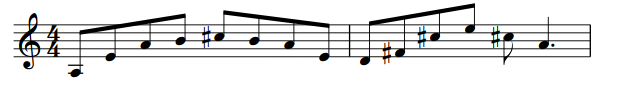
\includegraphics[width=.85\linewidth]{../code/musikla/musikla/examples/paper/concatenation2.png}}%
  }%
  \caption{Generated music sheet for concatenation\protect\footnotemark.}
  \label{fig:concatenation}
\end{figure}

\footnotetext{Rendered with \$ABC\_UI. Some hand made changes made for clarity.}


\paragraph*{Repetition}
The repetition operand is in a way very similar to the concatenation operator. It makes sense, since repeating any kind of music pattern $N$ times could be thought as a particular case of as concatenation where there are $N$ operands, all representing the same musical pattern.

\begin{lstlisting}[caption={Intro to Westworld's Theme by Ramin Djawadi},label=list:8-6,captionpos=t,abovecaptionskip=-\medskipamount]
I1 S6/8 T140 L/8 V90;
A*11 G F*12
\end{lstlisting}

\begin{figure}[h]
  \centering
  {%
  \setlength{\fboxsep}{0pt}%
  \setlength{\fboxrule}{0pt}%
  \fbox{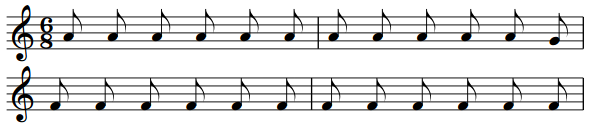
\includegraphics[width=.85\linewidth]{../code/musikla/musikla/examples/paper/repetition2.png}}%
  }%
  \caption{Generated music sheet for repetition.}
  \label{fig:repetition}
\end{figure}

\paragraph*{Parallel}
The parallel operator enables playing multiple sequences of musical events simultaneously. However our events are emitted as a single sequence of ordered events, thus requiring merging the multiple sequences into a single one, while maintaining the properties of laziness and order. The operator assumes that each of its operands already maintains those properties on their own, and so is only in charge of making sure the merged sequence does so as well. With this in mind, it relies on a custom \textit{merge sorted} algorithm for iterables (not related to the most common merge sort algorithm by John von Neumann).

\begin{lstlisting}[caption={Snippet of Soft to Be Strong by Marina},label=list:8-6,captionpos=t,abovecaptionskip=-\medskipamount]
T120 V70 L1;
[^Cm] [BM] | r/4 ^g/4 ^g/4 ^f/2 e/8 ^d3/8 ^c
\end{lstlisting}

\begin{figure}[h]
  \centering
  {%
  \setlength{\fboxsep}{0pt}%
  \setlength{\fboxrule}{0pt}%
  \fbox{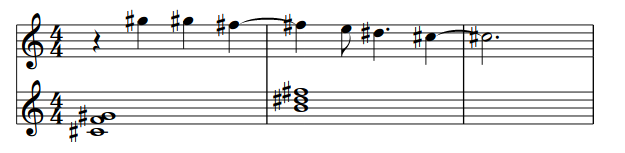
\includegraphics[width=.85\linewidth]{../code/musikla/musikla/examples/paper/parallel.png}}%
  }%
  \caption{Generated music sheet for parallel}
  \label{fig:parallel}
\end{figure}

The merge sorted function receives $N$ operands and creates a buffer with the size $N$. For each operand it \textit{forks} the context, so that they can execute concurrently and each will mutate their own context only. It then requests one single event for each operand.

After the buffer is prefilled (meaning it has at least one event for all non-empty operands), the algorithm finds the earliest event stored in the it. Let's assume it is stored in the $K$ index of the buffer, with $K < N$. The method emits the value stored in \texttt{buffer[K]} and then fills requests the next event from the $K$ operand (storing \texttt{null} if the operand has no more events to emit). It then repeats this step until all operands have been drained.

\subsection{Integration in a Programming Environment}
Apart from generating musical events from somewhat static instructions, our goal is to have those events integrate into a programming language in the same way integers, floats, strings and booleans do: as data that can be stored, passed around and manipulated. This, of course, must still retain all the properties we've laid out for our sequences of events: being lazy and always being ordered.

\paragraph*{Variables and Functions}
Up until now we've analyzed situations where the timing of the events is known at the moment of their creation (through inspection of the context passed onto them). However, there can be situations where the events have to be created before their time location is known.

We decided to take an approach to integrate this type of functionality that does not require different semantics for creating events \textit{"live"} and for storing events in all operators. Instead, the only changes occur in variable declarations and when inserting variables in the middle of other expressions.

When declaring a variable, its expression is evaluated with custom context, forked from the main context, with the cursor reset back to zero. An important thing to note is that even though we are storing the music in a variable, we still take care to respect the principle of laziness present throughout our language: when the variable is declared, no actual events are created. Later, whenever the variable is used, and an event is requested of the variable, it relays that request to the expression responsible for providing the event.

However, one important caveat is that the variable cannot simply emit the events as they are created, because as we mentioned before, their context is a different one from the main context (with its cursor set to zero at the start of the expression).

Let's assume that a variable $C$ holds the value of the \texttt{cursor(ctx)}, it \texttt{ctx} is the context where the variable is being evaluated (not declared). Then, each event would be cloned and its starting time would have the constant $C$ added to it.

This raises an important detail that we must not forget: many of the musical events are created and then emitted directly. However, as we've seen, some can be stored in variables. And variables can be used in many ways, and the same variable can be used multiple times. This means that if one were to mutate an event (by change its start time or its duration, for instance), we would be changing the the contents of the variable. This could be an acceptable approach. But we have opted instead for a more functional approach, treating those musical events as more akin to primitive values (as we would treat numbers or event strings in modern languages). This means that when we change the start time of an event, we are actually cloning it.

This works well enough because those events are very lightweight objects, and the benefits of not having their values mysteriously changed outweight the small cost of a possible unnecessary allocation, in case that event was actually only used once.

\paragraph*{Functions}
When designing functions into our language, we decided to keep the semantics simple. Emitting events inside a function is similar to its return value being an iterator that gives out the emitted events on demand. This means that a value cannot both emit musical events, while also returning other values manually through a return statement.

There is no syntactic marker to distinguish regular functions from musical-emitting ones. Instead, the language runtime starts executing each function as a regular one, and automatically switches its execution mode into a generator-like implementation once the first event is emitted. Any return statements that are evaluated after this point must have no value (thus preserving the feature to early-stop a function). If they do try to return a custom value, a runtime exception is triggered.

In terms of managing the implicit context, functions are treated in very similar ways to the regular operators. They receive the context that was active at their call site and are evaluated with it. This means that any events emitted will have begin at whatever time the context's cursor marks.

Their arguments, however, are treated the same way as variable declarations (which is what they really are), meaning that each argument gets a custom fork of the call site's context with its \texttt{cursor} set to zero.

Here we can see a small snippet of the beginning of Fugue 2 in C minor in Book I of the J.S. Bach’s Well-Tempered Clavier, and how using functions can help us visualize the structure behind music.

\begin{lstlisting}[caption={Example of repeating the same note},label=list:8-6,captionpos=t,abovecaptionskip=-\medskipamount]
fun fugue ( $subj, $resp ) => 
    ( $subj $resp | stretch( r, $subj ) ( $subj + 7 ) );

S8/4 T140 L/4 V120;

$subj = r c/2 B/2 c G _A c/2 B/2 c d
        G c/2 B/2 c d F/2 G/2 _A2 G/2 F/2;

$resp = E/2 c/2 B/2 A/2   G/2 F/2 _E/2 D/2   C _e d c
        _B A _B c   ^F G _A F;

play( fugue( $subj, $resp ) );
\end{lstlisting}


\begin{figure}[h]
  \centering
  {%
  \setlength{\fboxsep}{0pt}%
  \setlength{\fboxrule}{0pt}%
  \fbox{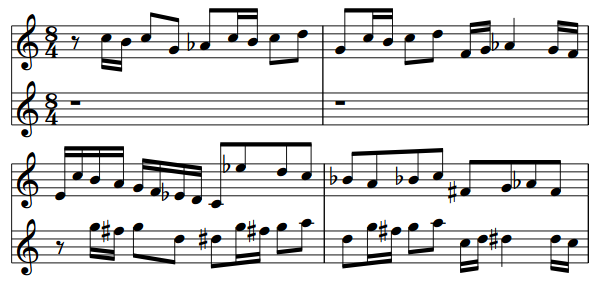
\includegraphics[width=.85\linewidth]{../code/musikla/musikla/examples/paper/fugue.png}}%
  }%
  \caption{Generated music sheet for fugue example}
  \label{fig:parallel}
\end{figure}
% https://drive.google.com/open?id=1-igVwdhXMxOSE1cMg_8HimDOXMhsY9US


\section{Results Discussion}
\label{sec:conclusions}

To solve our problem of keeping track of the timing implicitly for each event created, we decided to pass around a context variable. There were other possible solutions, like keeping this data in some sort of global variable. Our approach does give us some advantages, such as beeing able to have multiple contexts in play at the same time. It does have drawbacks, too. Every function defined in our language must receive this context to be able to create events at the appropriate time. However, functions defined in Python do not expect this parameter. Therefore, special conversions must be made when exchanging values between both languages.

Also, our solution to have variables just offset the timings of each event they contain every time those variables are used simplifies the process of integrating variables into our existing semantics of music generation. This solution, however, does not answer other questions unrelated to the timing, such as: should events stored in variables use the musical instrument set when they were declared, or when the variable was used?

However, this early work already provides a solid foundation for a musical \textit{DSL} that while dynamic (with variables, functions and control structures) integrates very well with established musical standards such as the MIDI protocol and others.


\bibliography{references}

\end{document}
